\documentclass{IOS-Book-Article}
\usepackage{mathptmx}
\usepackage{soul}\setuldepth{article}
\usepackage{times}
\usepackage{graphicx} 
\usepackage{booktabs}
\usepackage{makecell}

\normalfont
\usepackage[T1]{fontenc}

\def\hb{\hbox to 11.5 cm{}}
\begin{document}

\pagestyle{headings}
\def\thepage{}
\begin{frontmatter}

\title{Monitoring adherence to PBM guidelines from clinical data warehouse: a case study}

\markboth{}{October 2025\hb}

\author[A]{\fnms{Paul-Antoine} \snm{BEAUDOIN}},
\author[A]{\fnms{Alexandre} \snm{GODON}},
\author[A]{\fnms{Sebastien} \snm{MARQUET}},
\author[A]{\fnms{Thomas} \snm{BOULIER}%
\thanks{Corresponding Author: Thomas Boulier, E-mail: tboulier@chu-grenoble.fr.}}, 
and
\author[A]{\fnms{Alexandre} \snm{MOREAU-GAUDRY}}

\runningauthor{P.-A. Beaudoin et al.}
\address[A]{Univ. Grenoble Alpes, CNRS, UMR 5525, VetAgro Sup, Grenoble INP, CHU Grenoble Alpes, TIMC, 38000 Grenoble, France}

\begin{abstract}
Despite strong evidence, implementing Patient Blood Management (PBM) in routine practice remains 
challenging. This work describes the method we used at Grenoble Alpes University Hospital for 
producing quality reports using data from a graph-based clinical data warehouse.
\end{abstract}

\begin{keyword}
Patient Blood Management\sep Clinical data warehouse\sep Graph database \sep Health information system
\end{keyword}
\end{frontmatter}

\markboth{October 2025\hb}{October 2025\hb}

\section{Introduction}

Patient Blood Management (PBM) is an evidence-based, multidisciplinary approach to
optimize patient care and reduce unnecessary transfusion. 
It relies on three pillars: detection and correction of preoperative anemia, reduction 
of perioperative blood loss, and optimization of anemia tolerance. 
It has demonstrated effectiveness in reducing 
transfusions \cite{godonReductionRedBlood2024}, yet variability in adherence across 
departments persists and scaling implementation requires continuous monitoring and feedback.
This addresses a key challenge in health informatics: integrating information 
technology within real healthcare systems to support continuous quality improvement.

In France, the \textit{If-PBM} program was introduced to support the implementation of PBM 
through targeted funding.  One of its key requirements is to develop dashboards for monitoring 
adherence to PBM guidelines, providing funded centers with tools to track progress and identify areas
for improvement.

\section{Methods}

Five indicators were computed every three months: the proportion of standardized PBM preoperative check-ups,
 the proportion of corrective treatments for anemia or iron deficiency, the proportion of patients 
 transfused per- or postoperatively, the proportion of single-unit transfusion episodes, and the 
 proportion of patients discharged with low hemoglobin levels. Each indicator was calculated for 3 
 specific surgical specialties: orthopedics, cardiology, and gynecology. 

PBM indicators were computed quarterly from our graph-based clinical data warehouse \cite{Artemova2019}
using Talend-orchestrated Python pipelines linking patients, transfusions, lab tests, and surgical 
procedures.

\section{Results}

The PBM monitoring system has been operational since May 2023, with quarterly 
reports deployed across three surgical specialties. Over a two-year period, an 
average of 353 surgeries per quarter were analyzed (orthopedics: 170, 
cardiology: 132, gynecology: 75).

As an example, Figure~\ref{fig:pbm_trends} illustrates the temporal evolution of preoperative 
PBM assessment completion rates. Overall compliance increased from 40\% in May 
2023 to 80\% in February 2025. Orthopedics showed the fastest improvement, 
reaching 90\% by August 2023 from 30\% in May 2023, while gynecology remained under
60\% throughout the period.

\begin{figure}[h!]
\vspace{-1em}
\centering
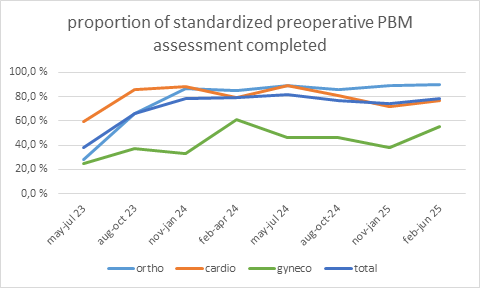
\includegraphics[width=0.85\textwidth]{figure.png}
\caption{Temporal trends of standardized preoperative PBM assessment completion rates by surgical specialty (May 2023 -- February 2025). The graph shows quarterly measurements for orthopedics (blue), cardiology (orange), gynecology (green), and overall hospital performance (dark blue).}
\label{fig:pbm_trends}
\vspace{-1em}
\end{figure}

\section{Discussion}

Our automated reports identified departments requiring targeted PBM education 
(e.g., gynecology for preoperative assessments). We plan to implement targeted micro-learning modules,
using these automated reports as the primary, objective criterion to evaluate their effectiveness.

Future developments involve refactoring the current stack with modern tools (Dagster, dbt, OMOP) as part of a regional 
initiative to deploy fully automated, web-accessible dashboards.

\begin{thebibliography}{99}

\bibitem{godonReductionRedBlood2024}
Godon A, Dupuis M, Amdaa S, Pevet G, Girard E, Fiard G, Sourd D, Bosson JL, Payen JF, Albaladejo P, Bouzat P. Reduction of red blood cell transfusion with a patient blood management protocol in urological and visceral surgery: A before-after study. Anaesthesia Critical Care \& Pain Medicine. 2024 Aug;43(4):101395.

\bibitem{Artemova2019}
Artemova S, Madiot PE, Moreau-Gaudry A, et al. PREDIMED: Clinical Data Warehouse of Grenoble Alpes University Hospital. In: MEDINFO 2019: Health and Wellbeing e-Networks for All. 2019. p. 1421--1425.

\end{thebibliography}

\end{document}